\documentclass[11pt]{article}
\usepackage[margin=.73in]{geometry}
\usepackage{lmodern,amsmath,amssymb,booktabs,graphicx,microtype,fancyhdr,xurl,hyperref,array}
\hypersetup{colorlinks=true,urlcolor=blue,linkcolor=black,pdftitle={HPS GPR v6.4.3: Global probabilities with shifted signal MC}}
\pagestyle{fancy}\fancyhf{}\lhead{HPS GPR: global probabilities with signal MC}\rhead{v6.4.3}\cfoot{\thepage}
\setlength{\headheight}{14pt}\setlength{\parindent}{0pt}\setlength{\parskip}{6pt}\setlength{\emergencystretch}{2em}
\begin{document}
{\LARGE\bfseries Global probabilities\par with the selected signal-MC windows}\par
{\large 2016, 2021 and their combined analysis}\par
25 September 2026\hfill Version 6.4.3

\textbf{The result.} With the 2016 fit and GP-training exclusion set to $[-2.5,+2.5]u$, its largest observed excess statistic occurs at 91 MeV. The largest statistics for 2021 and for the combined analysis occur at 67 MeV. Complete background-only simulations give the mass-scan global probabilities below. Each result uses 1,024 independent simulated experiments, and every experiment is searched over the entire corresponding mass grid.

\begin{center}\small\begin{tabular}{lrrrrr}\toprule
Search & Peak [MeV] & Exceedances & Global $p$ & 95\% MC interval & Global $Z$\\\midrule
2016 & 91 & 67/1024 & 0.066 & [0.051, 0.082] & 1.50\\
2021 & 67 & 239/1024 & 0.234 & [0.208, 0.261] & 0.73\\
Combined & 67 & 202/1024 & 0.198 & [0.173, 0.223] & 0.85\\
\bottomrule\end{tabular}\end{center}

The 2016 local asymptotic value of $3.46\sigma$ becomes $1.50\sigma$ globally; the combined value changes from $2.83\sigma$ to $0.85\sigma$. All three global values are below $2\sigma$ under this calibration.

The quoted $p$ is the add-one estimate $(k+1)/1025$; the interval describes finite-simulation uncertainty in the background exceedance probability. $Z=\max[0,\Phi^{-1}(1-p)]$ expresses the same probability in positive-excess Gaussian units. The probability itself is always reported, including when $Z$ clips to zero.

\textbf{The selected models and mass searches.} Define $u=(m_{\rm rec}-c(m))/s(m)$ using the interpolated MC core center $c$ and width $s$. The MC displacement is already contained in the signal template.

\begin{center}\small\begin{tabular}{lll}\toprule
Search & Signal model and fit/training exclusion & Mass grid [MeV]\\\midrule
2016 & Neighbor MC; $[-2.5,+2.5]u$ & 40--175, step 1\\
2021 & Neighbor MC; $[-4,+3]u$ & 60--240, step 1\\
Combined & Same MC models; retain 2015 Gaussian & 60--240, step 1\\\bottomrule
\end{tabular}\end{center}

The observations are the archived full 2015 and 2016 spectra and the archived 2021 10\% spectrum. The combined fit uses one common signal-strength parameter. All three campaigns contribute through 100 MeV; 2016 and 2021 contribute at 101--175 MeV; only 2021 contributes at 176--240 MeV. Consequently, the combined search is not an all-three-campaign search over its entire domain.

\textbf{If the largest result among these three searches is selected.} A supplementary calibration maximizes the same statistic over all three displayed searches as well as mass. It gives $k=102$ of 1,024, $p=0.100$, with a 95\% interval [0.082, 0.120] and $Z=1.28$. Correlations are retained because each simulated campaign spectrum is reused in all searches that contain that campaign.

These are conditional global probabilities for the stated grids and a fixed GP background source estimated from the observed spectra. They include the search over mass, but not uncertainty in that source or the earlier choice among windows and signal models. Those limits on interpretation are part of the result.

\clearpage\section*{Exactly what is repeated in a simulated search?}

\textbf{Signal shapes and normalization.} The 2016 template comes from the target-constrained, FEE-smeared and scaled histograms \texttt{h\_MinvScSm\_GeneralLargeBins\_Final\_1}. The 2021 template uses the saved v16 target-constrained MC bank. The saved local Gaussian-plus-affine core fits define the centers and widths; the full empirical histograms define the signal shapes. Between neighboring simulated masses, the core centers and widths are interpolated linearly; the full histogram cumulative probabilities are aligned in $u$ and mixed with the same linear weights. Bin probabilities are differences of this cumulative distribution. At an anchor the original selected MC distribution is recovered. Neither year is extrapolated beyond its adopted MC domain.

Bin centers determine fit membership. The GP is trained on the exterior of the same interval, with no additional excluded region. In 2016, the actual fit bins contain 94.52--97.42\% of the full selected template. The template is not renormalized to this interval: its tails and any probability outside the stored spectrum remain part of its normalization. The 2015 Gaussian and its original $\pm2.25\sigma_{\rm ref}$ interval are retained.

\textbf{The fitted statistic.} The GP uses the training-bin counts to predict the mean background $b$ and covariance in the excluded bins. In count space, write the expected fitted counts as
\[
 \lambda=b+L\eta+\psi S,\qquad \eta\sim N(0,I),\qquad \psi=\epsilon^2/10^{-8}.
\]
Here $LL^\mathsf{T}$ is the regularized GP covariance and $S$ is the binned full-template signal multiplied by the inherited campaign-specific yield conversion. The fit uses Poisson counts and the Gaussian constraint on $\eta$, with positive expected counts. For the combination, campaign background constraints are independent while $\psi$ is common. The free fitted strength is signed. At each mass,
\[
 r(m)=\operatorname{sign}(\widehat\psi)\sqrt{2[\ell(0)-\ell(\widehat\psi)]},
 \qquad q_0(m)=\max[0,r(m)]^2,\qquad T=\max_{m\in\mathcal M}q_0(m),
\]
where $\ell$ is the nuisance-profiled negative log likelihood. The observed peak is selected by this raw statistic, not by a mass-dependent calibrated local probability.

\textbf{The null source.} For each campaign, the archived source is the GP arithmetic-mean spectrum obtained from all observed bins using the saved kernel parameters at a 76 MeV reference mass. It is positive and has been reconstructed numerically from the frozen inputs. It is held fixed when generating independent Poisson counts in every bin. No latent GP function is drawn, and the source is not re-estimated between experiments.

\textbf{The repeated extraction.} A single full-spectrum count draw per campaign and experiment is reused at every mass and in every applicable search. At each mass, the selected exclusion is applied, the GP mean and covariance are recomputed from that draw, and both the free and zero-signal nuisance profiles are fitted. The mass-dependent archived kernel parameters, signal templates and yield conversions remain fixed. This preserves correlations between neighboring mass hypotheses without treating them as independent trials.

For $k$ simulated maxima at least as large as the observed maximum, we report $(k+1)/(N+1)$ alongside $k/N$ in the data tables and an exact two-sided 95\% Clopper--Pearson interval for the exceedance probability. The same simulations also give pointwise local tails. There is no subtraction of a null mean or rescaling of $r$ before constructing the scan maximum.

\clearpage\section*{From a local excess to a mass-scan probability}
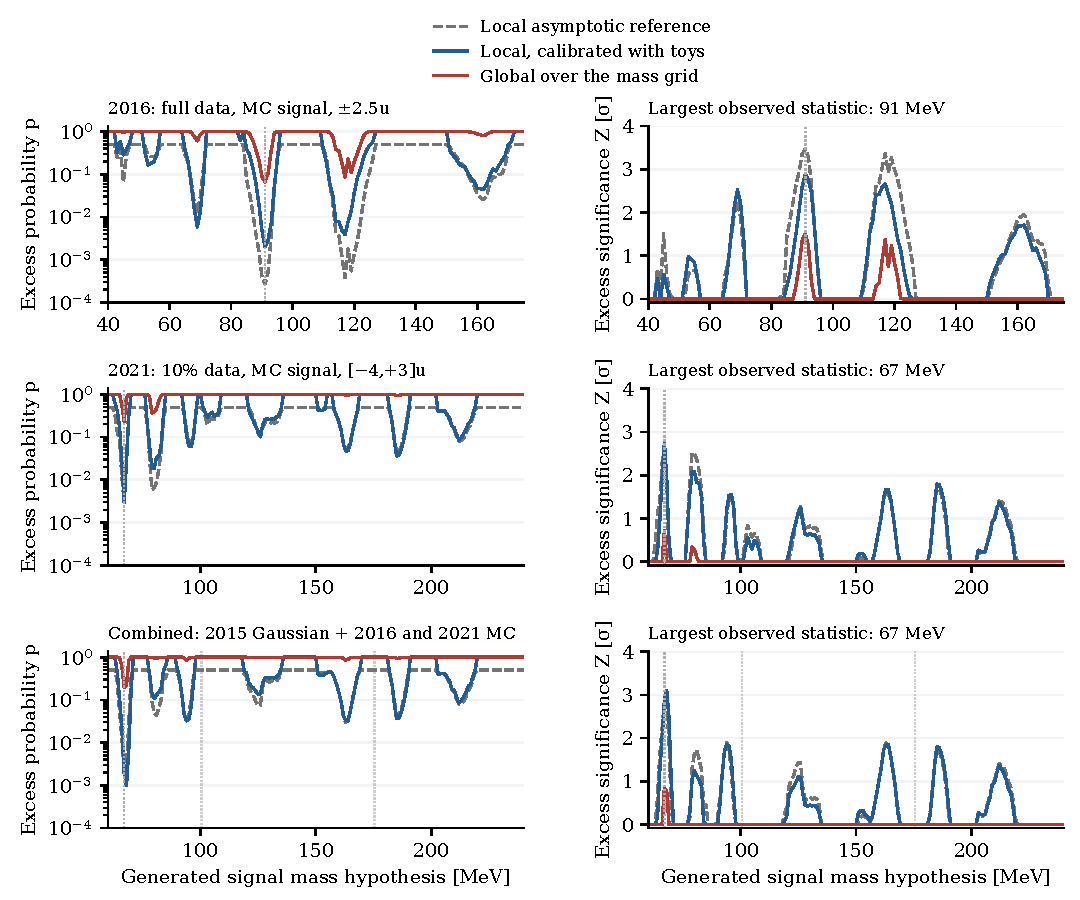
\includegraphics[width=\textwidth]{../figures/local_and_global_scans.pdf}
\refstepcounter{figure}\textbf{Figure \thefigure. How to read the three probability descriptions.} Gray is the inherited fixed-mass asymptotic reference, $p=\Phi[-\max(0,r)]$. Blue compares each observed $q_0(m)$ with simulated $q_0$ at that same mass. Red compares it with the largest simulated $q_0$ anywhere in the corresponding scan. The vertical line marks the largest observed raw statistic; dotted boundaries in the combined row mark changes in the contributing campaigns. All $Z$ values are clipped at zero for $p\ge1/2$; at $q_0=0$, the empirical upper tail includes all ties and equals one.

\begin{center}\small\begin{tabular}{lrrrrr}\toprule
At the selected peak & Asymptotic $Z$ & Local $k/N$ & Local toy $p$ & Local toy $Z$ & Global $Z$\\\midrule
2016 & 3.46 & 1/1024 & 0.0020 & 2.89 & 1.50\\
2021 & 2.74 & 2/1024 & 0.0029 & 2.76 & 0.73\\
Combined & 2.83 & 1/1024 & 0.0020 & 2.89 & 0.85\\
\bottomrule\end{tabular}\end{center}

The change from gray to blue tests the local reference distribution under this background source. The change from blue to red then includes the search over mass with the same raw statistic. Neither step assumes a number of independent resolution elements. The selected local tails have only one or two exceedances: their 95\% probability intervals are $[0.0000247,0.00543]$ for 2016 and combined, and $[0.000237,0.00704]$ for 2021. Thus small differences between local asymptotic and toy values are not resolved precisely by this sample.

\clearpage\section*{The distribution of the largest background excess}
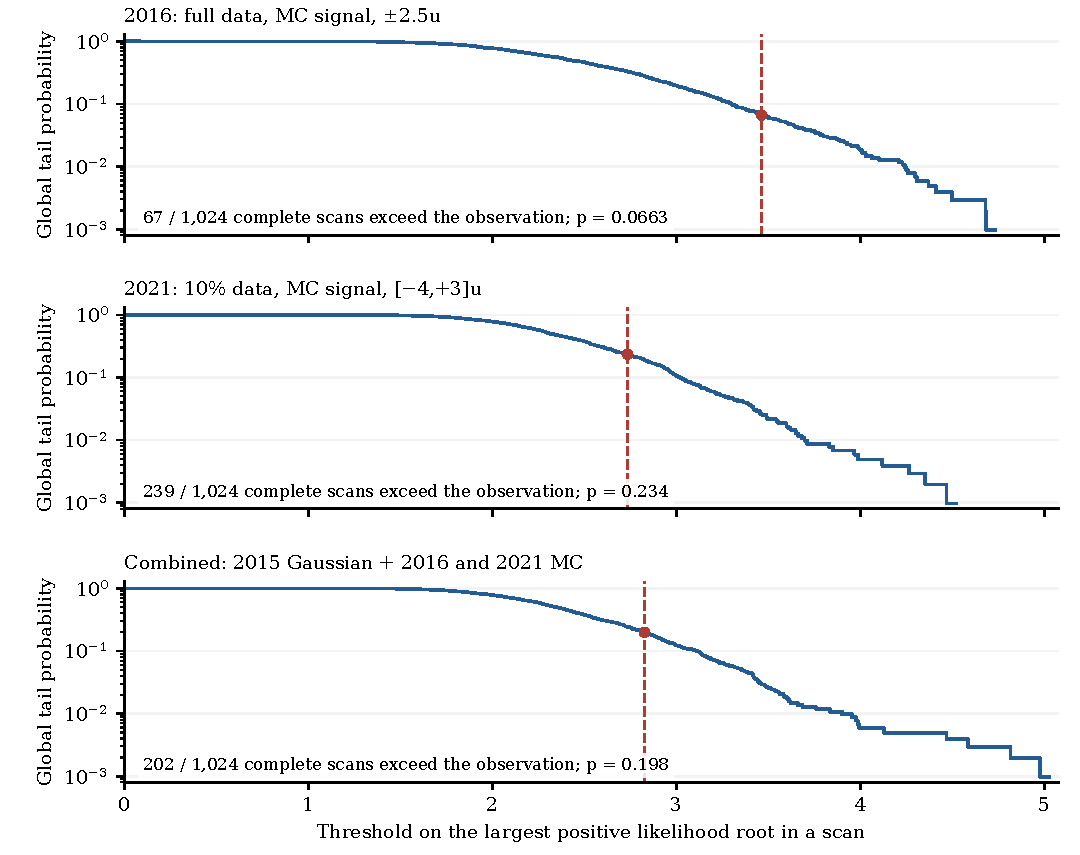
\includegraphics[width=\textwidth]{../figures/scan_maximum_tails.pdf}
\refstepcounter{figure}\textbf{Figure \thefigure. The global probabilities are measured directly.} Blue shows the add-one upper tail of the largest positive likelihood root in each of the 1,024 complete simulated searches. The red line is the observed maximum, and its intersection with the blue curve gives the reported global probability. The finite-simulation floor is $1/1025$; the curve is not extrapolated into an unmeasured tail.

\begin{center}\small\begin{tabular}{lrrr}\toprule
Search & Observed peak [MeV] & Null mean of $r$ at that mass & Null standard deviation\\\midrule
2016 & 91 & +0.648 & 0.957\\
2021 & 67 & +0.093 & 1.027\\
Combined & 67 & -0.031 & 0.968\\
\bottomrule\end{tabular}\end{center}

These pointwise moments help interpret the difference between asymptotic and simulated local probabilities. They are diagnostics of the chosen GP source and extraction, and are not used to recenter the statistic. The global calibration includes their effect automatically. Its finite-simulation interval describes uncertainty from the number of experiments, not uncertainty in the background model or detector response.

\clearpage\section*{Scope, validation and reproducibility}

\textbf{What the probabilities answer.} Under each fixed archived background source, how often would the selected extraction produce a largest excess statistic at least as large as the one observed on its stated 1 MeV grid? The three primary rows answer that question separately. The supplementary family probability also allows choosing among these three displayed searches. It does not include selecting the 2016 window from the earlier $\pm3.5u$, $\pm2u$ and current $\pm2.5u$ alternatives, changing the template family, or selecting a different background construction.

Because the null source was estimated from the same observed spectra, this study conditions on that estimate. It does not propagate uncertainty in the source or demonstrate that any real signal would be excluded from its construction. The result is also restricted to the finite mass grid; a continuously optimized mass search would require its own calibration. The 2021 input remains the 10\% data sample, without an extrapolation to full luminosity. These calculations therefore do not establish an unconditional physical discovery significance.

\textbf{Relation to the preceding studies.} The neighboring-template construction, archived spectra, kernel settings and common-strength likelihood are inherited from the v6.3.n and v6.4.n studies. This note selects $\pm2.5u$ for 2016 and recomputes the observed scans and their null calibration. The previous $\pm3.5u$ extraction and $\pm2u$ appendix remain preserved. Their upper limits retain those earlier windows; no previous upper-limit curve is relabeled as a $\pm2.5u$ result. This note reports significance rather than a new limit calibration.

\textbf{Numerical validation.} All 169 frozen input files are verified by SHA-256. The saved arrays contain 1,024 complete experiments at all 136 2016 masses and all 181 masses in each of the 2021 and combined searches, with no failed or discarded fit rows. This corresponds to 443,392 distinct pairs of free and zero-signal profile fits; the combined result above 175 MeV reuses the identical 2021 fit. Maximum score residual was $2.00\times10^{-7}$ and the smallest fitted expected bin count was 120.10. Every expected count was positive.

Validation regenerated every campaign draw from its seed, checked the complete mass arrays against their checkpoints, verified the fit/exclusion masks and full-template normalization, reconstructed all three null sources, and independently replayed 60 saved toy profiles at eight representative masses. All 181 observed 2021 likelihood roots reproduce the preceding MC extraction to within $4.14\times10^{-10}$. The scan maxima, exceedance counts, confidence intervals and family combination were recomputed from the saved arrays. Previously delivered reports were preserved.

\textbf{Files needed to reproduce or inspect the result.} The accompanying source package contains the inputs, protocol hashes, executable scripts, complete toy scan arrays, per-mass checkpoints, figure data and this LaTeX source. \texttt{README.md} gives the bounded two-worker rebuild command. The numerical tables are \texttt{results/global\_summary.csv} and \texttt{results/local\_global\_curves.csv}; \texttt{results/toy\_maxima.csv} records every simulated maximum. \texttt{qa/global\_validation.json} records the numerical checks. The checkpoint signature pins the sample count, random seed, inputs and extraction code, so a resumed run cannot silently mix different analyses.

\textbf{Precision.} The fixed sample size was chosen before calibration. The add-one tail has resolution $1/1025$; 1,024 experiments cannot establish an extremely small tail probability. Zero exceedances, if encountered, would give a finite upper bound and never zero probability or infinite significance. No additional simulations were selected according to the observed calibration tail.
\end{document}
